\documentclass[a4paper,openright,12pt]{book}
\usepackage[spanish,es-nodecimaldot]{babel}
\usepackage[utf8]{inputenc}
\usepackage[T1]{fontenc}
\usepackage{lmodern}
\usepackage{amsmath,amssymb,amsfonts}
\usepackage{graphicx}
\usepackage{float}
\usepackage{booktabs}
\usepackage{setspace}
\usepackage{geometry}
\usepackage{microtype}
\usepackage[hypertexnames=false,hidelinks]{hyperref}
\usepackage{cite}
\usepackage{caption}
\usepackage{enumitem}

\geometry{margin=2.5cm}
\onehalfspacing
\setcounter{secnumdepth}{3}
\setcounter{tocdepth}{2}
\captionsetup{font=small,labelfont=bf}

\begin{document}

%======================================================================
\begin{titlepage}
\begin{center}
\vspace*{0.4cm}
{\large UNIVERSIDAD DE LOS ANDES}\\[0.35cm]
{\large FACULTAD DE CIENCIAS}\\[0.25cm]
{\large DEPARTAMENTO DE F\'ISICA APLICADA}\\[1.6cm]

{\LARGE\bfseries An\'alisis variacional Kramers--Kronig restringido\\[0.25cm]
de espectros \'opticos:\\[0.35cm]
modelado de la funci\'on diel\'ectrica\\[0.15cm]
y validaci\'on de constantes \'opticas}\\[1.4cm]

\rule{70mm}{0.4pt}\\[1.0cm]

\begin{tabular}{ll}
Autor: & Golfredo P\'erez Fern\'andez \\[0.35cm]
Tutor: & Juan Mart\'in \\[0.35cm]
Cotutor: & --- \\
\end{tabular}

\vspace{2.2cm}
\textit{Trabajo de grado}\\[0.4cm]
M\'erida, Venezuela\\[0.2cm]
\today
\end{center}
\end{titlepage}

\frontmatter
\tableofcontents
\clearpage
\listoffigures

\chapter*{Resumen}
\addcontentsline{toc}{chapter}{Resumen}
La respuesta lineal de un s\'olido a un campo electromagn\'etico se describe mediante la funci\'on diel\'ectrica compleja
$\hat\varepsilon(\omega)=\varepsilon_1(\omega)+i\varepsilon_2(\omega)$.
De ella se derivan el \'indice de refracci\'on, la extinci\'on, la reflectividad, la absorci\'on y la conductividad \'optica.
En un experimento, por lo general se mide una de esas magnitudes en una ventana finita de frecuencias, no el par $(\varepsilon_1,\varepsilon_2)$ en todo el eje.
Este trabajo formula e implementa un an\'alisis variacional restringido por Kramers--Kronig: representa $\varepsilon_2$ mediante una base triangular, calcula $\varepsilon_1$ con la transformada anal\'itica de esa base y ajusta sus amplitudes con Levenberg--Marquardt para reproducir la magnitud medida.
Adem\'as, establece criterios para evaluar consistencia algebraica, causalidad, fidelidad a los datos y sensibilidad a las cantidades que el experimento no determina.
La tesis se organiza en tres partes: fundamentos y Seminario~I; m\'etodo e implementaci\'on f\'isica y Seminario~II; y criterios de validaci\'on, alcance y limitaciones.

\vspace{0.8cm}
\noindent\textbf{Palabras clave:} funci\'on diel\'ectrica, Kramers--Kronig, an\'alisis variacional, espectroscop\'ia \'optica, Levenberg--Marquardt.

\chapter*{Abstract}
\addcontentsline{toc}{chapter}{Abstract}
The linear optical response of a solid is described by its complex dielectric function.
This thesis formulates and implements a Kramers--Kronig constrained variational analysis: it represents the imaginary part with triangular basis functions, obtains the real part from their analytic transforms, and fits the measured optical quantity with Levenberg--Marquardt.
It also defines tests for algebraic consistency, causality, data fidelity, and sensitivity to quantities that the measurement does not determine. Its conclusions are limited to the evidence and assumptions stated for each test.

\mainmatter
%======================================================================
\part{Fundamentos de la respuesta \'optica\\y Seminario I}
%======================================================================

\chapter{El problema cient\'ifico}
\label{ch:problema}

\section{Motivaci\'on}

Cuando la radiaci\'on electromagn\'etica atraviesa o refleja en un s\'olido, el material no responde de manera instant\'anea ni local en el sentido microsc\'opico m\'as general.
Macrosc\'opicamente, sin embargo, esa respuesta puede condensarse en unas pocas funciones de frecuencia.
Entre ellas, la funci\'on diel\'ectrica compleja es el objeto central:
contiene la informaci\'on sobre polarizaci\'on, absorci\'on, retardos de fase y, en \'ultima instancia, sobre excitaciones electr\'onicas, fonones, excitones y portadores libres~\cite{electrodynamics,MarkFox}.

El experimentalista suele medir una sola magnitud proyectada:
reflectividad a incidencia normal~$R(\omega)$,
coeficiente de absorci\'on~$\alpha(\omega)$,
transmitancia de una l\'amina~$T(\omega)$,
o bien el \'indice~$n$ y la extinci\'on~$k$ en un intervalo limitado.
El problema inverso consiste en reconstruir $\hat\varepsilon(\omega)$ ---y con ella el resto del espectro \'optico--- sin imponer un modelo microsc\'opico r\'igido del tipo Lorentz, Tauc--Lorentz o Fano, que puede sesgar la interpretaci\'on cuando la muestra no cabe en esas formas.

\section{Planteamiento formal}

En un medio lineal, homog\'eneo e is\'otropo (redes c\'ubicas, por simplicidad), el desplazamiento el\'ectrico y el campo el\'ectrico se relacionan en el dominio de Fourier por
\begin{equation}
\mathbf{D}(\omega)=\hat\varepsilon(\omega)\,\mathbf{E}(\omega),
\qquad
\hat\varepsilon(\omega)=\varepsilon_1(\omega)+i\varepsilon_2(\omega).
\end{equation}
La conductividad \'optica compleja $\hat\sigma(\omega)=\sigma_1(\omega)+i\sigma_2(\omega)$ es equivalente, en unidades gaussianas,
\begin{equation}
\label{eq:eps-sigma}
\hat\varepsilon(\omega)=1+\frac{4\pi i}{\omega}\hat\sigma(\omega).
\end{equation}
La causalidad ---el material no responde antes de que llegue el campo--- implica que $\varepsilon_1$ y $\varepsilon_2$ no son independientes: quedan ligados por las relaciones de Kramers--Kronig~\cite{Jackson,electrodynamics}:
\begin{align}
\label{eq:kk1}
\varepsilon_1(\omega)-1
&=\frac{2}{\pi}\,\mathcal{P}\!\int_{0}^{\infty}
\frac{x\,\varepsilon_2(x)}{x^{2}-\omega^{2}}\,dx,\\
\label{eq:kk2}
\varepsilon_2(\omega)
&=-\frac{2\omega}{\pi}\,\mathcal{P}\!\int_{0}^{\infty}
\frac{\varepsilon_1(x)-1}{x^{2}-\omega^{2}}\,dx
+\frac{4\pi\sigma_{\mathrm{dc}}}{\omega}.
\end{align}
Aqu\'i $\mathcal{P}$ denota el valor principal de Cauchy y $\sigma_{\mathrm{dc}}$ es la conductividad continua.

Si se midiera $\varepsilon_2(\omega)$ en todo el eje, $\varepsilon_1$ quedar\'ia fijada.
En el laboratorio el eje es finito.
Lo que queda fuera de la ventana experimental se resume en un fondo de alta frecuencia $\varepsilon_\infty$, y lo que queda dentro debe parametrizarse de forma flexible pero causal.
Ese es el n\'ucleo del an\'alisis variacional restringido de Kuzmenko~\cite{constrained}.

\section{Objetivos}

\paragraph{Objetivo general.}
Formular y demostrar, paso a paso, un procedimiento f\'isico completo para modelar la funci\'on diel\'ectrica compleja a partir de espectros \'opticos medibles mediante an\'alisis variacional Kramers--Kronig restringido, e implementar ese procedimiento en una aplicaci\'on de an\'alisis espectral que permita validar la consistencia de los resultados.

\paragraph{Objetivos espec\'ificos.}
\begin{enumerate}[leftmargin=*]
\item Derivar, desde las ecuaciones de Maxwell, las constantes \'opticas relevantes y sus v\'inculos con $\hat\varepsilon$.
\item Exponer el an\'alisis variacional con base triangular y la minimizaci\'on por Levenberg--Marquardt.
\item Especificar c\'omo cada magnitud medible ($R$, $T$, $\alpha$, $n$, $k$, $\varepsilon_1$, $\varepsilon_2$) entra en el funcional $\chi^{2}$.
\item Validar que los resultados reconstruidos son f\'isicamente verdaderos en el sentido de causalidad, pasividad, reproducci\'on de datos y consistencia cruzada entre constantes.
\end{enumerate}

\section{Alcance}

Se trabaja en respuesta lineal, medios no magn\'eticos ($\mu=1$), incidencia normal desde el vac\'io y, salvo indicaci\'on contraria, muestras semi-infinitas o l\'aminas en aire con reflexiones m\'ultiples incoherentes.
No se tratan aqu\'i elipsometr\'ias anisotr\'opicas ni multicapas arbitrarias sobre sustrato.
La luminiscencia se discute solo como emisi\'on: su intensidad no es $\varepsilon_2$ y no define un par Kramers--Kronig.

\section{Organizaci\'on de la tesis}

La \textbf{Parte~I} desarrolla el marco electromagn\'etico y culmina en el Seminario~I.
La \textbf{Parte~II} detalla el m\'etodo variacional, el ajuste y la f\'isica de cada medida; culmina en el Seminario~II.
La \textbf{Parte~III} presenta criterios de verdad experimental y resultados de validaci\'on.


\chapter{Marco electromagn\'etico}
\label{ch:marco}

\section{Ecuaciones de Maxwell en medios}

En unidades gaussianas, las ecuaciones macrosc\'opicas leen~\cite{Jackson}
\begin{align}
\nabla\cdot\mathbf{D}&=4\pi\rho_{\mathrm{lib}},&
\nabla\cdot\mathbf{B}&=0,\\
\nabla\times\mathbf{E}&=-\frac{1}{c}\frac{\partial\mathbf{B}}{\partial t},&
\nabla\times\mathbf{H}&=\frac{4\pi}{c}\mathbf{J}_{\mathrm{lib}}
+\frac{1}{c}\frac{\partial\mathbf{D}}{\partial t}.
\end{align}
Para campos arm\'onicos $e^{-i\omega t}$ y constitutivas lineales
$\mathbf{D}=\hat\varepsilon\mathbf{E}$, $\mathbf{B}=\mathbf{H}$ (no magn\'etico) y $\mathbf{J}=\hat\sigma\mathbf{E}$,
se recupera la relaci\'on~\eqref{eq:eps-sigma}.
La funci\'on diel\'ectrica y la conductividad son dos lenguajes de la misma respuesta.

\section{Propagaci\'on y \'indice complejo}

La ecuaci\'on de onda en el medio introduce el \'indice de refracci\'on complejo
$\hat N(\omega)=n(\omega)+ik(\omega)$ mediante
\begin{equation}
\hat N^{2}(\omega)=\hat\varepsilon(\omega).
\end{equation}
Separando partes real e imaginaria,
\begin{equation}
\label{eq:eps-nk}
\varepsilon_1=n^{2}-k^{2},\qquad
\varepsilon_2=2nk.
\end{equation}
La inversi\'on estable es
\begin{equation}
\label{eq:nk-from-eps}
n=\sqrt{\frac{|\varepsilon|+\varepsilon_1}{2}},\qquad
k=\sqrt{\frac{|\varepsilon|-\varepsilon_1}{2}},
\end{equation}
con $|\varepsilon|=\sqrt{\varepsilon_1^{2}+\varepsilon_2^{2}}$.
En un medio pasivo, $\varepsilon_2\ge 0$ y se toma $k$ con el mismo signo que $\varepsilon_2$.

El coeficiente de absorci\'on, con n\'umero de onda $\tilde\nu=\omega/(2\pi c)$ en cm$^{-1}$, es
\begin{equation}
\label{eq:alpha}
\alpha=4\pi\tilde\nu\,k.
\end{equation}
La conductividad \'optica en $\Omega^{-1}\mathrm{cm}^{-1}$ admite la forma pr\'actica~\cite{electrodynamics}
\begin{equation}
\label{eq:sigma}
\sigma_1=\frac{\tilde\nu\,\varepsilon_2}{60},\qquad
\sigma_2=\frac{\tilde\nu\,(\varepsilon_\infty-\varepsilon_1)}{60}.
\end{equation}

\section{Reflectividad a incidencia normal}

Para un medio semi-infinito iluminado desde el vac\'io a incidencia normal, el coeficiente de reflexi\'on de amplitud es
\begin{equation}
\label{eq:r-complex}
\hat r=\frac{1-\hat N}{1+\hat N}=\sqrt{R}\,e^{i\phi}.
\end{equation}
La reflectividad de intensidad resulta
\begin{equation}
\label{eq:R}
R=\frac{(n-1)^{2}+k^{2}}{(n+1)^{2}+k^{2}}.
\end{equation}
Esta expresi\'on no describe una pel\'icula sobre sustrato ni una l\'amina con dos caras coherentes: para esos casos hace falta espesor e \'indices del entorno~\cite{OpticalTechniques}.

La ruta cl\'asica de an\'alisis Kramers--Kronig sobre $R(\omega)$ recupera la fase $\phi$ mediante
\begin{equation}
\phi(\omega)=-\frac{2\omega}{\pi}\,\mathcal{P}\!\int_{0}^{\infty}
\frac{\ln\sqrt{R(x)}}{x^{2}-\omega^{2}}\,dx+\phi(0),
\end{equation}
e invierte~\eqref{eq:r-complex} para obtener $\hat\varepsilon$.
Esa ruta es correcta en incidencia normal, pero no se generaliza sin esfuerzo a otras geometr\'ias.
El an\'alisis variacional restringido trabaja directamente sobre $\varepsilon_2$ y proyecta cualquier magnitud \'optica causal, lo que lo hace m\'as vers\'atil~\cite{constrained}.

\begin{figure}[H]
\centering
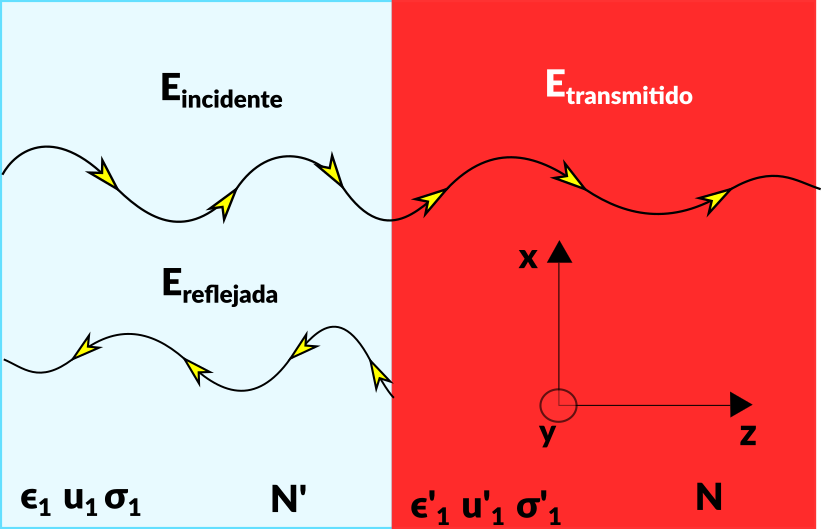
\includegraphics[width=0.85\textwidth]{reflectividadNormal.png}
\caption{Esquema de radiaci\'on a incidencia normal sobre una superficie: rayos incidente, reflejado y transmitido.}
\label{fig:incid-normal}
\end{figure}

\section{Transmitancia de una l\'amina}

Para una l\'amina de espesor $d$ en aire, sumando reflexiones m\'ultiples incoherentes,
\begin{equation}
\label{eq:T}
T=\frac{(1-R)^{2}x}{1-R^{2}x^{2}},
\qquad
x=e^{-\alpha d}=e^{-4\pi\tilde\nu k\,d},
\end{equation}
y la absorbancia decadica (densidad \'optica)
\begin{equation}
A=-\log_{10}T.
\end{equation}
Sin espesor no hay $T$ ni $A$ bien definidos desde el modelo.

\section{Funci\'on de p\'erdida}

La funci\'on de p\'erdida de energ\'ia
\begin{equation}
-\mathrm{Im}\!\left(\frac{1}{\hat\varepsilon}\right)
=\frac{\varepsilon_2}{\varepsilon_1^{2}+\varepsilon_2^{2}}
\end{equation}
resalta modos longitudinales y el plasm\'on.
Un $\varepsilon_\infty$ demasiado bajo infla artificialmente esta magnitud porque $|1/\varepsilon|$ crece.

\section{Procesos \'opticos en el s\'olido}

En distintos rangos espectrales dominan mecanismos distintos~\cite{MarkFox,Ashcroft}:
\begin{itemize}[leftmargin=*]
\item infrarrojo lejano y medio: fonones y portadores libres (Drude);
\item visible y ultravioleta cercano: transiciones interbanda, excitones;
\item energ\'ias a\'un mayores: contribuciones que, vistas desde una ventana limitada, se aglomeran en $\varepsilon_\infty$.
\end{itemize}

\begin{figure}[H]
\centering
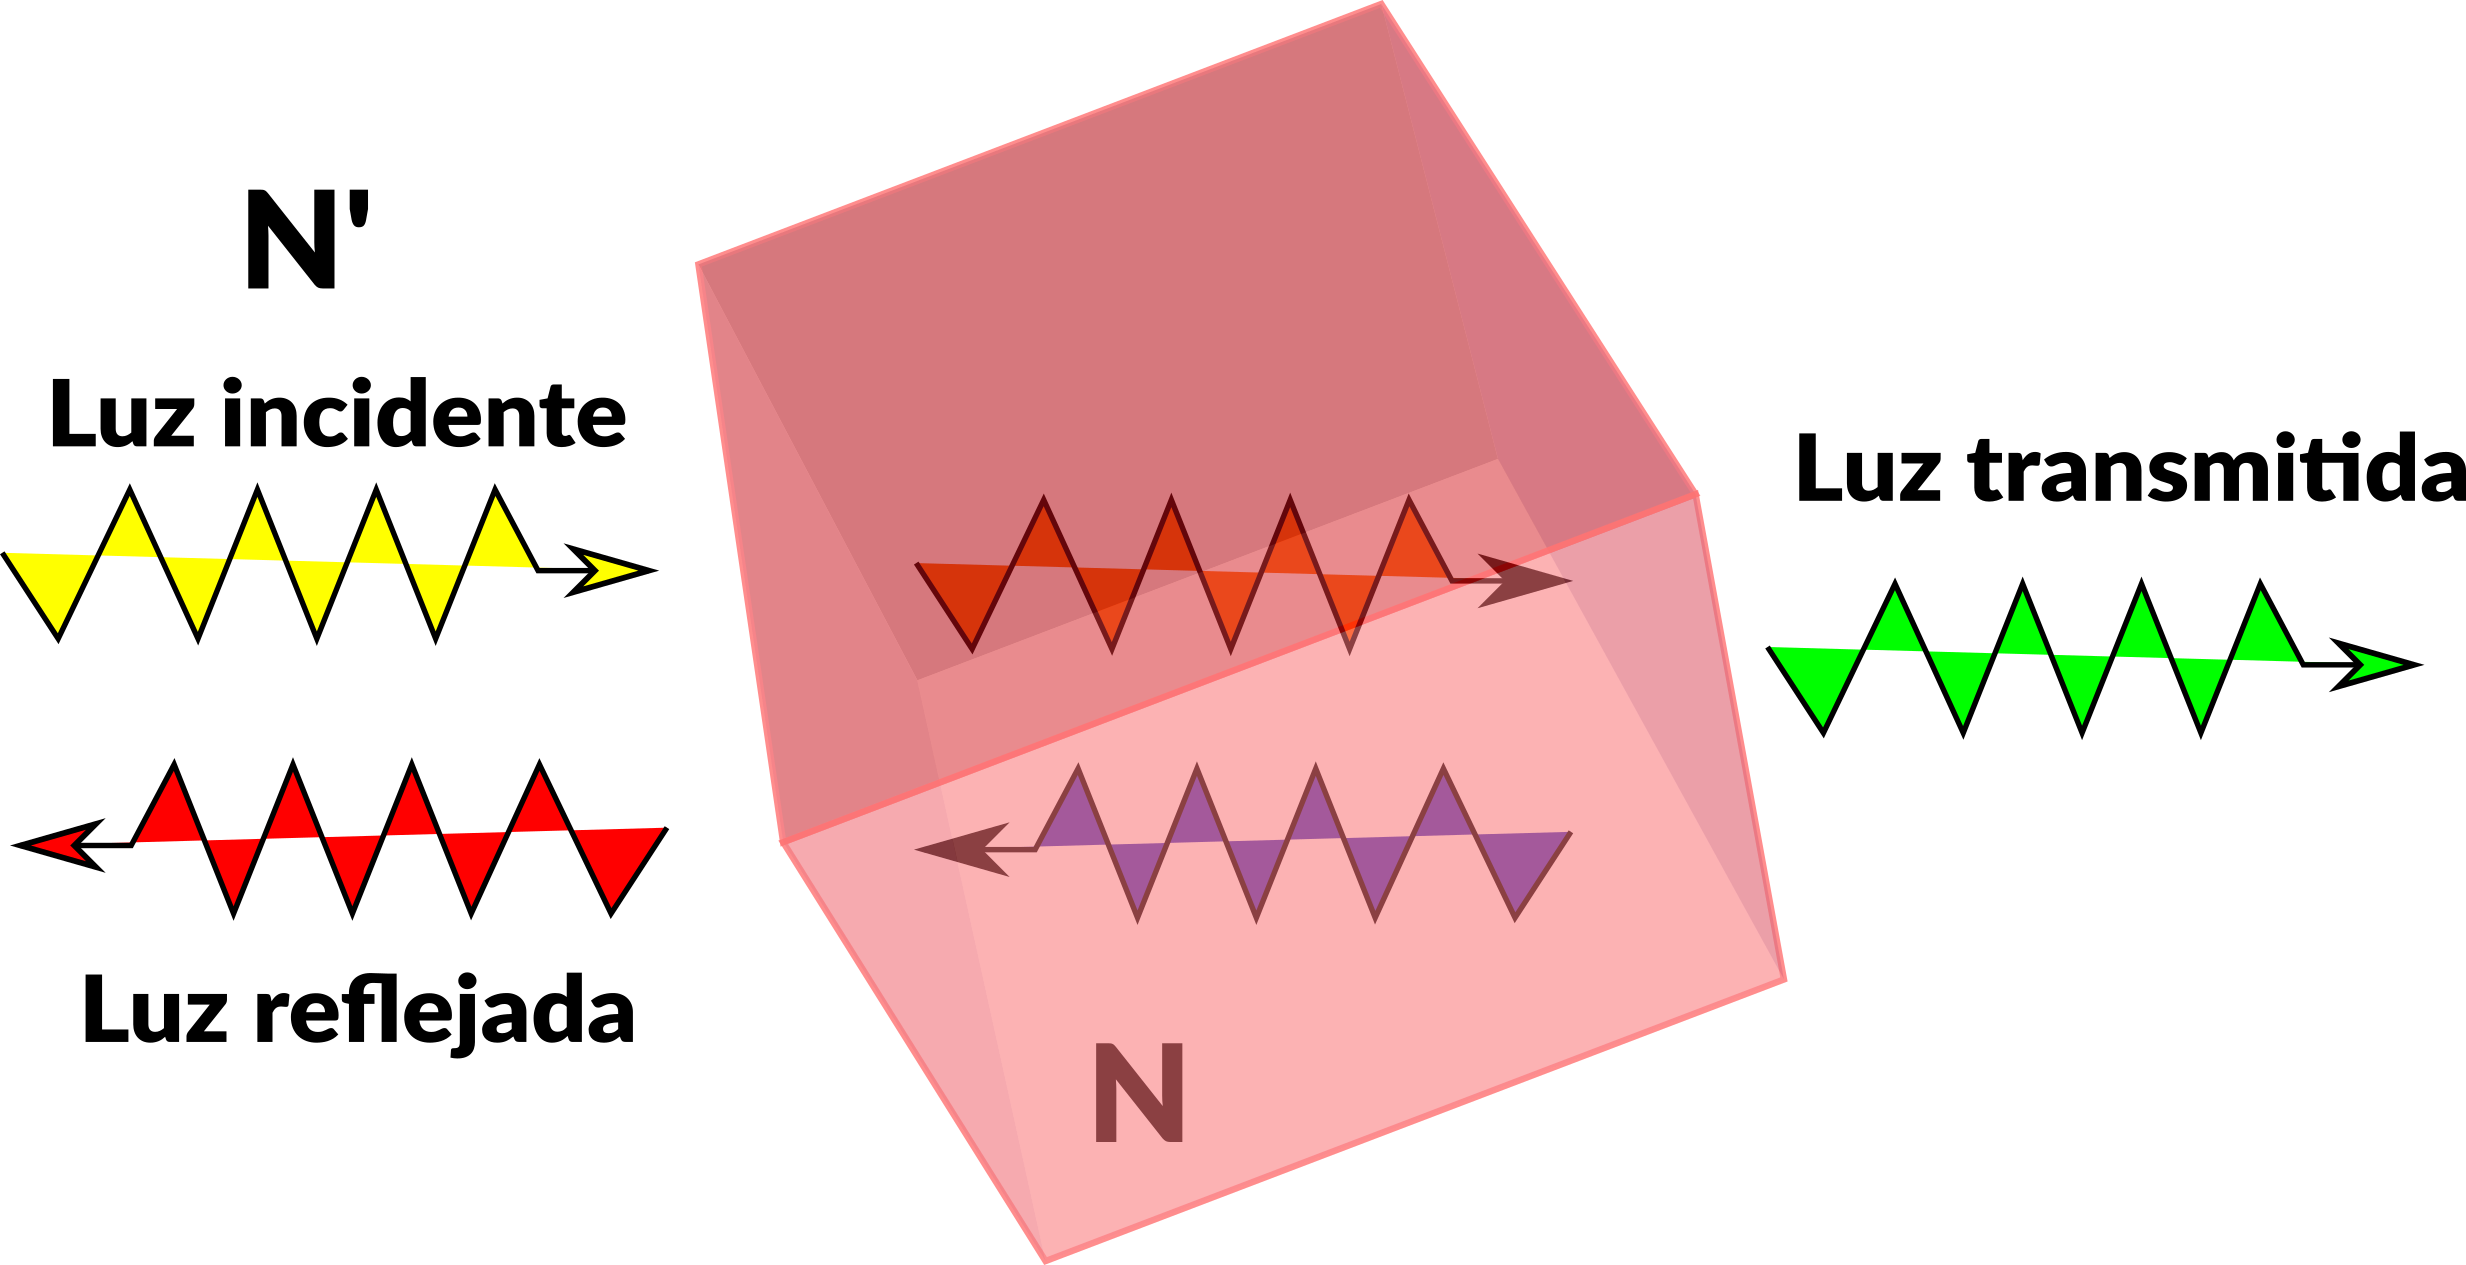
\includegraphics[width=0.88\textwidth]{procesosopticos.png}
\caption{Clasificaci\'on esquem\'atica de procesos \'opticos seg\'un la escala de energ\'ia.}
\label{fig:procesos}
\end{figure}

El modelo de Drude para electrones libres,
\begin{align}
\label{eq:drude}
\varepsilon_{2,\mathrm{D}}&=\frac{\omega_p^{2}\gamma\omega}{\omega^{4}+\gamma^{2}\omega^{2}},\\
\varepsilon_{1,\mathrm{D}}&=\varepsilon_\infty-\frac{\omega_p^{2}\omega^{2}}{\omega^{4}+\gamma^{2}\omega^{2}},
\end{align}
describe el fondo met\'alico.
En el an\'alisis variacional puede restarse antes de ajustar los tri\'angulos, de modo que las anclas describan el resto del espectro~\cite{constrained}.


\chapter{Causalidad y relaciones Kramers--Kronig}
\label{ch:kk}

\section{De la respuesta temporal a la frecuencia}

Si la polarizaci\'on es
\begin{equation}
\mathbf{P}(t)=\int_{-\infty}^{t}\chi(t-t')\,\mathbf{E}(t')\,dt',
\end{equation}
la funci\'on de respuesta $\chi(\tau)$ se anula para $\tau<0$.
En frecuencia, $\hat\varepsilon(\omega)=1+4\pi\hat\chi(\omega)$ es anal\'itica en el semiplano superior (con convenciones habituales), y las relaciones~\eqref{eq:kk1}--\eqref{eq:kk2} siguen del teorema de Cauchy~\cite{Jackson}.

\begin{figure}[H]
\centering
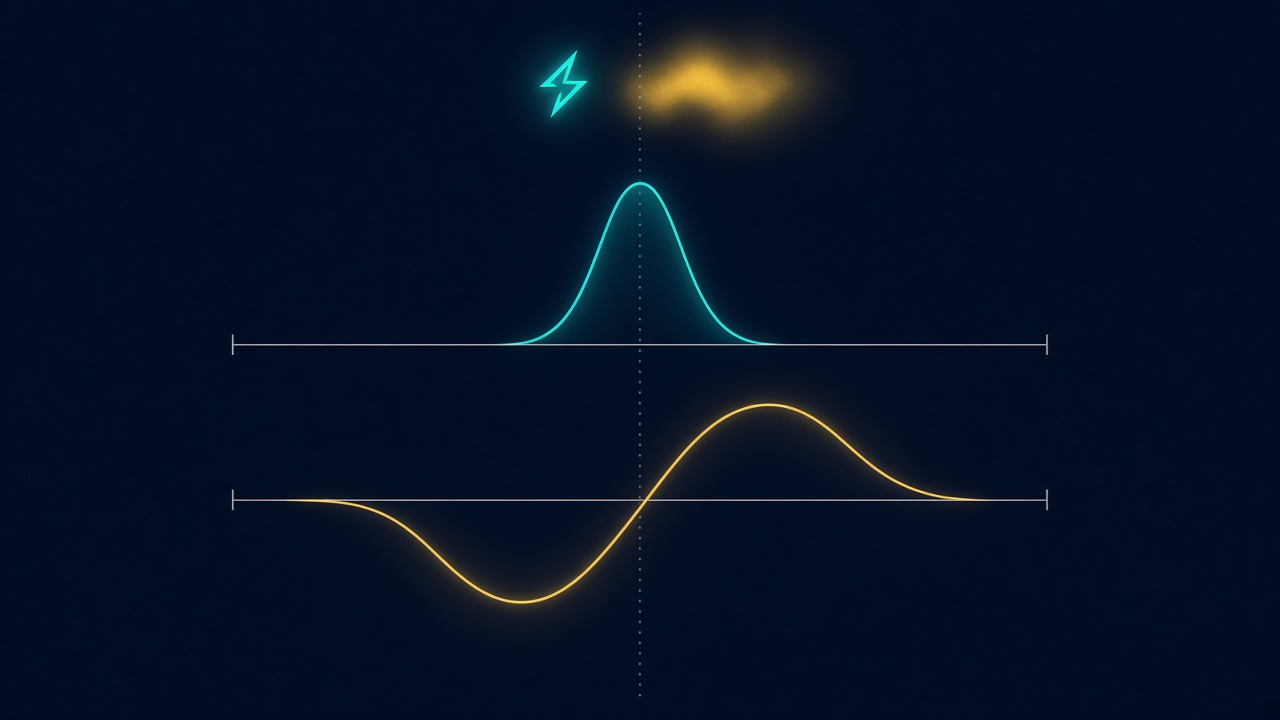
\includegraphics[width=0.82\textwidth]{learn-kk.jpg}
\caption{Un pico de absorci\'on en $\varepsilon_2$ fija la forma dispersiva de $\varepsilon_1$: no son dos ajustes independientes.}
\label{fig:kk-pair}
\end{figure}

\section{Ventana experimental y $\varepsilon_\infty$}

La integral Kramers--Kronig requiere, en principio, todo el eje.
En la pr\'actica se escribe
\begin{equation}
\label{eq:eps1-window}
\varepsilon_1(\omega)
=\varepsilon_\infty
+\frac{2}{\pi}\,\mathcal{P}\!\int_{\omega_{\min}}^{\omega_{\max}}
\frac{x\,\varepsilon_2(x)}{x^{2}-\omega^{2}}\,dx
+\text{(colas)},
\end{equation}
donde $\varepsilon_\infty$ recoge la contribuci\'on de altas frecuencias no medidas.
Interpretaci\'on operativa:
\begin{itemize}[leftmargin=*]
\item si el usuario fija $\varepsilon_\infty$, ese valor se respeta;
\item si se mide $n$ o $\varepsilon_1$, $\varepsilon_\infty$ puede ajustarse junto con las alturas de $\varepsilon_2$;
\item si se mide $R$ y $\varepsilon_\infty$ no se da, puede estimarse del extremo de alta frecuencia asumiendo $k$ peque\~no:
$n=(1+\sqrt{R})/(1-\sqrt{R})$, $\varepsilon_\infty=n^{2}$;
\item si se mide $k$, $\alpha$ o $T$, la magnitud no fija $\varepsilon_\infty$; el valor por defecto~$1$ reproduce bien $\alpha$ y $k$, pero no necesariamente $n$ ni $R$.
\end{itemize}

\section{Pasividad}

Un medio pasivo exige $\varepsilon_2(\omega)\ge 0$.
En el ajuste se puede penalizar $\varepsilon_2$ negativa para no abandonar el dominio f\'isico.
Esa penalizaci\'on es una regularizaci\'on f\'isica, no un dato experimental adicional.


\chapter*{Seminario I\\Respuesta \'optica lineal y la funci\'on diel\'ectrica}
\addcontentsline{toc}{chapter}{Seminario I}
\label{sem:1}

\noindent\textit{Parte~I --- exposici\'on de seminario.}

\section*{S.I.1 Prop\'osito}

Este seminario resume, para un auditorio de f\'isica de materiales, el contenido necesario antes de hablar de ajuste num\'erico:
qu\'e es $\hat\varepsilon$, c\'omo se conecta con lo que se mide, y por qu\'e Kramers--Kronig no es un adorno matem\'atico sino una ley de causalidad.

\section*{S.I.2 Mensaje central}

\begin{enumerate}[leftmargin=*]
\item Toda magnitud \'optica lineal de inter\'es puede escribirse en t\'erminos de $\varepsilon_1$ y $\varepsilon_2$ (o de $n$ y $k$).
\item Medir una sola proyecci\'on no basta, en general, para fijar el par completo sin hip\'otesis adicionales.
\item La causalidad suministra esa hip\'otesis: conocida $\varepsilon_2$ en un eje suficientemente amplio, $\varepsilon_1$ queda determinada salvo el fondo $\varepsilon_\infty$ de lo no medido.
\item Por tanto, el problema bien planteado es: \emph{buscar el $\varepsilon_2$ causal cuyo par Kramers--Kronig reproduce la magnitud experimental}.
\end{enumerate}

\section*{S.I.3 Demostraci\'on guiada (pizarra)}

\begin{enumerate}[leftmargin=*]
\item Partir de $\hat N^{2}=\hat\varepsilon$ y obtener~\eqref{eq:eps-nk}.
\item Invertir a~\eqref{eq:nk-from-eps}.
\item Sustituir en~\eqref{eq:R} y discutir el l\'imite transparente $k\to 0$.
\item Enunciar~\eqref{eq:kk1} e interpretar el pico de $\varepsilon_2$ frente a la dispersi\'on an\'omala de $\varepsilon_1$.
\item Se\~nalar el papel de $\varepsilon_\infty$ como ``todo lo que no cabe en la ventana''.
\end{enumerate}

\section*{S.I.4 Criterio de \'exito del seminario}

Al final, el auditorio debe poder responder sin ambig\"uedad:
\begin{itemize}[leftmargin=*]
\item qu\'e se gana al obtener $\hat\varepsilon$ frente a quedarse solo con $R$ o $\alpha$;
\item por qu\'e un ajuste independiente de $\varepsilon_1$ y $\varepsilon_2$ puede violar causalidad;
\item qu\'e hip\'otesis f\'isicas entran al estimar $\varepsilon_\infty$ desde $R$ en el extremo alto.
\end{itemize}

\section*{S.I.5 Puente hacia la Parte~II}

El Seminario~II tratar\'a c\'omo construir $\varepsilon_2$ con tri\'angulos, c\'omo evaluar $\varepsilon_1$ en forma cerrada y c\'omo minimizar $\chi^{2}$ sin abandonar Kramers--Kronig en ning\'un paso.

%======================================================================
\part{\texorpdfstring{M\'etodo variacional, implementaci\'on f\'isica\\y Seminario II}{Metodo variacional, implementacion fisica: Seminario II}}
%======================================================================

\chapter{An\'alisis variacional Kramers--Kronig restringido}
\label{ch:variacional}

\section{Idea del m\'etodo}

En lugar de ajustar un modelo microsc\'opico con pocos polos, se representa $\varepsilon_2(\omega)$ como superposici\'on de funciones base triangulares centradas en anclas de frecuencia fijas~\cite{constrained}:
\begin{equation}
\label{eq:eps2-tri}
\varepsilon_2(\omega)=\sum_{k=1}^{M}A_k\,\Lambda_k(\omega)
+\varepsilon_{2,\mathrm{D}}(\omega),
\end{equation}
donde $\Lambda_k$ vale $1$ en la ancla $\omega_k$, cae linealmente a $0$ en las anclas vecinas y es nula fuera de ese soporte. Si $\omega_0<\omega_1<\cdots<\omega_M<\omega_{M+1}$, con amplitudes nulas en los extremos $\omega_0$ y $\omega_{M+1}$, cada base se define como
\begin{equation}
\Lambda_k(\omega)=
\begin{cases}
\dfrac{\omega-\omega_{k-1}}{\omega_k-\omega_{k-1}},&\omega_{k-1}\le\omega\le\omega_k,\\[6pt]
\dfrac{\omega_{k+1}-\omega}{\omega_{k+1}-\omega_k},&\omega_k<\omega\le\omega_{k+1},\\[6pt]
0,&\text{fuera de ese intervalo.}
\end{cases}
\end{equation}
El t\'ermino $\varepsilon_{2,\mathrm{D}}$ es un fondo Drude opcional; al desactivarlo vale cero.
Los par\'ametros libres son las alturas $A_k$ (y, cuando procede, $\varepsilon_\infty$).

La parte real se obtiene por Kramers--Kronig \emph{exacta} de esa parametrizaci\'on:
\begin{equation}
\label{eq:eps1-tri}
\varepsilon_1(\omega)
=\varepsilon_\infty
+\sum_{k=1}^{M}A_k\,K_k(\omega)
+\bigl[\varepsilon_{1,\mathrm{D}}(\omega)-\varepsilon_\infty\bigr],
\end{equation}
donde $K_k$ es la transformada de Kramers--Kronig del tri\'angulo unitario $\Lambda_k$.
As\'i, en cada iteraci\'on del ajuste el par $(\varepsilon_1,\varepsilon_2)$ es causal por construcci\'on.

\begin{figure}[H]
\centering

\includegraphics[width=0.88\textwidth]{learn-triangles.jpg}
\caption{Base triangular: cada ancla aporta un ``sombrero'' a $\varepsilon_2$; su pareja dispersiva entra en $\varepsilon_1$ con pesos cerrados.}
\label{fig:triangles}
\end{figure}

\section{N\'ucleo anal\'itico del tri\'angulo}

Para obtener $K_k$, se sustituye un tri\'angulo en la relaci\'on de Kramers--Kronig de $\varepsilon_2$. Definamos los espaciamientos $\Delta_- = \omega_k-\omega_{k-1}$ y $\Delta_+ = \omega_{k+1}-\omega_k$. Al separar las dos pendientes del tri\'angulo, la integral queda
\begin{equation}
K_k(\omega)=\frac{2}{\pi}\mathcal{P}\left[
\frac{1}{\Delta_-}\int_{\omega_{k-1}}^{\omega_k}\frac{x(x-\omega_{k-1})}{x^2-\omega^2}\,dx
+\frac{1}{\Delta_+}\int_{\omega_k}^{\omega_{k+1}}\frac{x(\omega_{k+1}-x)}{x^2-\omega^2}\,dx
\right].
\end{equation}
La integral de cada tramo produce logaritmos. Para escribir el resultado de forma compacta, se define
\begin{equation}
G(x,y)=(x+y)\ln|x+y|-(x-y)\ln|x-y|,
\end{equation}
donde el t\'ermino $0\ln 0$ se toma por su l\'imite, igual a cero. La suma de los dos tramos es
\begin{equation}
K_k(\omega)=\frac{1}{\pi}\left[
\frac{G(\omega,\omega_{k-1})}{\Delta_-}
-\frac{\Delta_-+\Delta_+}{\Delta_-\Delta_+}G(\omega,\omega_k)
+\frac{G(\omega,\omega_{k+1})}{\Delta_+}
\right].
\end{equation}
Aunque cada logaritmo contiene una frecuencia dimensional, cualquier escala de referencia com\'un se cancela en esta combinaci\'on. Por tanto, en cada iteraci\'on no hace falta volver a integrar num\'ericamente: basta calcular $K_k$ y sumar las contribuciones $A_kK_k$.

\section{Malla de anclas y colas}

Las anclas se colocan de forma densa en picos y valles del espectro y se reparte el resto del intervalo medido. La selecci\'on conserva primero los extremos locales y luego distribuye anclas en el resto de la malla.
Fuera de la primera y la \'ultima ancla interior se a\~naden extremos con coeficiente nulo, de modo que $\varepsilon_2$ baja en l\'inea recta hasta cero.
Esa cola no est\'a fijada por los datos y puede desplazar $\varepsilon_1$ dentro de la ventana; por eso $\varepsilon_\infty$ y la extrapolaci\'on deben declararse con claridad al reportar resultados.

Cuando la magnitud medida no es $\varepsilon_2$ sino $R$, $T$, $n$, $k$ o $\alpha$, el n\'umero de anclas se limita al orden de cientos porque $\varepsilon_1$ en cada punto acopla globalmente las alturas. No se requiere una ancla por dato: todas las mediciones, sean o no anclas, entran en $\chi^{2}$.
En la implementaci\'on descrita aqu\'i se permiten hasta 500 anclas para espectros de hasta 5400 puntos; por encima de ese tama\~no se usan hasta 400 para respetar el presupuesto de c\'omputo a 800 iteraciones. Esta es una decisi\'on num\'erica de la implementaci\'on, no un requisito general del m\'etodo.

\section{Funcional a minimizar}

Dados $N$ puntos $\{(\omega_i,y_i,\sigma_i)\}$, se define el chi-cuadrado de los datos
\begin{equation}
\label{eq:chi2}
\chi^{2}_{\mathrm{datos}}=\sum_{i=1}^{N}
\left(\frac{y_i-Q\bigl(\omega_i;\{A_k\},\varepsilon_\infty\bigr)}{\sigma_i}\right)^{2},
\end{equation}
donde $Q$ es la magnitud declarada por el experimentalista, calculada desde el par $(\varepsilon_1,\varepsilon_2)$ del modelo.
Si no se suministra error, $\sigma_i=1$.

El ajuste minimiza un objetivo regularizado $\Phi$:
\begin{itemize}[leftmargin=*]
\item \textbf{suavidad:} $P_s=\lambda_s\sum_k(A_{k-1}-2A_k+A_{k+1})^2$ sobre tripletas interiores libres. La diferencia no se divide por el espaciamiento entre anclas; por ello, el efecto de la penalizaci\'on depende de la malla.
\item \textbf{negatividad:} $P_-=\lambda_-\sum_i\min(0,\varepsilon_2(\omega_i))^2$, que penaliza valores negativos del modelo en los puntos medidos.
\end{itemize}
As\'i, $\Phi=\chi^{2}_{\mathrm{datos}}+P_s+P_-$. Las penalizaciones participan en la minimizaci\'on, pero se excluyen del $\chi^{2}_{\mathrm{datos}}$ reportado como fidelidad a la medida.


\chapter{Minimizaci\'on: Levenberg--Marquardt}
\label{ch:lm}

\section{Gradiente y curvatura}

Sea $\mathbf{p}$ el vector de par\'ametros ($A_k$ y eventualmente $\varepsilon_\infty$).
El algoritmo de Levenberg--Marquardt interpola entre descenso por gradiente e inversi\'on de la curvatura~\cite{NR,guide}. Para ver de d\'onde sale el sistema lineal, definimos el residuo normalizado $r_i=(y_i-Q_i)/\sigma_i$. Cerca de los par\'ametros actuales, una variaci\'on peque\~na $\delta\mathbf{p}$ cambia la predicci\'on aproximadamente como
\begin{equation}
Q_i(\mathbf{p}+\delta\mathbf{p})\simeq Q_i(\mathbf{p})+\sum_l\frac{\partial Q_i}{\partial p_l}\,\delta p_l.
\end{equation}
Al sustituir esta aproximaci\'on lineal en la suma de cuadrados y minimizar respecto de $\delta\mathbf{p}$ se obtienen las ecuaciones normales. Las contribuciones de los datos al gradiente y a la curvatura de Gauss--Newton son
\begin{align}
\beta^{\mathrm{datos}}_k
&=-\frac12\frac{\partial\chi^{2}_{\mathrm{datos}}}{\partial p_k}
=\sum_i\frac{y_i-Q_i}{\sigma_i^{2}}\frac{\partial Q_i}{\partial p_k},\\
\alpha^{\mathrm{datos}}_{kl}
&=\sum_i\frac{1}{\sigma_i^{2}}
\frac{\partial Q_i}{\partial p_k}\frac{\partial Q_i}{\partial p_l},
\end{align}
Las penalizaciones aportan sus propias derivadas $\beta^{\mathrm{reg}}$ y curvatura $\alpha^{\mathrm{reg}}$; se combinan como $\beta=\beta^{\mathrm{datos}}+\beta^{\mathrm{reg}}$ y $\alpha\simeq\alpha^{\mathrm{datos}}+\alpha^{\mathrm{reg}}$. En cada iteraci\'on se amortigua la diagonal y se resuelve
\begin{equation}
\sum_l \alpha_{kl}(1+\lambda\delta_{kl})\,\delta p_l=\beta_k.
\end{equation}
Aqu\'i $\delta_{kl}$ es la delta de Kronecker: vale uno si $k=l$ y cero en otro caso. Se eval\'ua el objetivo $\Phi$ con los par\'ametros de prueba. Si disminuye, se acepta el paso y se reduce $\lambda$; si aumenta, se rechaza y se incrementa $\lambda$. As\'i, un $\lambda$ peque\~no aproxima Gauss--Newton, mientras uno grande produce pasos m\'as cautelosos, cercanos al descenso por gradiente.
Para $Q=\varepsilon_1$ o $\varepsilon_2$, las derivadas respecto de la funci\'on diel\'ectrica son directas. Para $Q=n$, $k$, $R$, $\alpha$ o $T$, la implementaci\'on estima $\partial Q/\partial\varepsilon_j$ mediante diferencias centrales; usa $h_j=10^{-6}(1+|\varepsilon_j|)$ para $j=1,2$.

\begin{figure}[H]
\centering
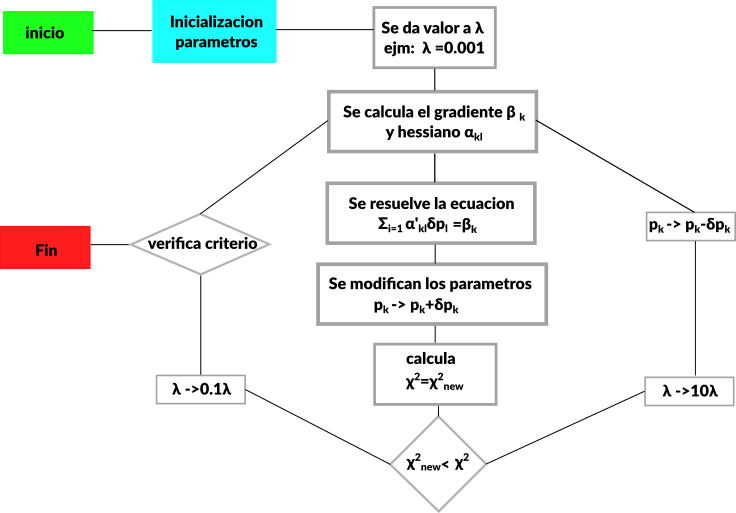
\includegraphics[width=0.78\textwidth]{diagrama.png}
\caption{Esquema del ciclo de Levenberg--Marquardt.}
\label{fig:lm}
\end{figure}

\section{Convergencia e incertidumbres}

En la implementaci\'on, una mejora menor al 1\% en $\Phi$ puede cerrar el ajuste solo cuando ning\'un residuo estandarizado supera el 2\% del rango total de la medida. Si el amortiguamiento crece sin reducir los residuos, el resultado se marca como estancado; alcanzar el m\'aximo de iteraciones tampoco equivale por s\'i solo a converger.
Cuando se suministran errores experimentales y el problema est\'a bien condicionado, la inversa de la curvatura de los datos $\alpha_{\mathrm{datos}}^{-1}$ permite estimar barras $\pm 1\sigma$ de los par\'ametros~\cite{NR}:
\begin{equation}
\delta p_k=\sqrt{(\delta\chi^{2}_{\mathrm{datos}})\,(\alpha_{\mathrm{datos}}^{-1})^{kk}}.
\end{equation}
Para intervalos de una desviaci\'on est\'andar se usa $\delta\chi^{2}_{\mathrm{datos}}=1$ cuando los errores declarados tienen interpretaci\'on estad\'istica. La estimaci\'on implementada excluye suavidad y penalizaci\'on de negatividad; por tanto, es condicional al modelo, a la malla y a los errores declarados, y no incluye toda la incertidumbre sistem\'atica ni la debida a extrapolar fuera de la ventana.
Un ejemplo muestra por qu\'e importa la correlaci\'on: con un solo dato $y=1$, $\sigma=1$ y $Q=p_1+p_2$, se obtiene $\chi^2=(1-p_1-p_2)^2$. Todos los pares con $p_1+p_2=1$ ajustan exactamente; el dato determina la suma, pero no cada par\'ametro por separado. Datos independientes o una restricci\'on f\'isica adicional hacen falta para separar sus valores.

\begin{figure}[H]
\centering
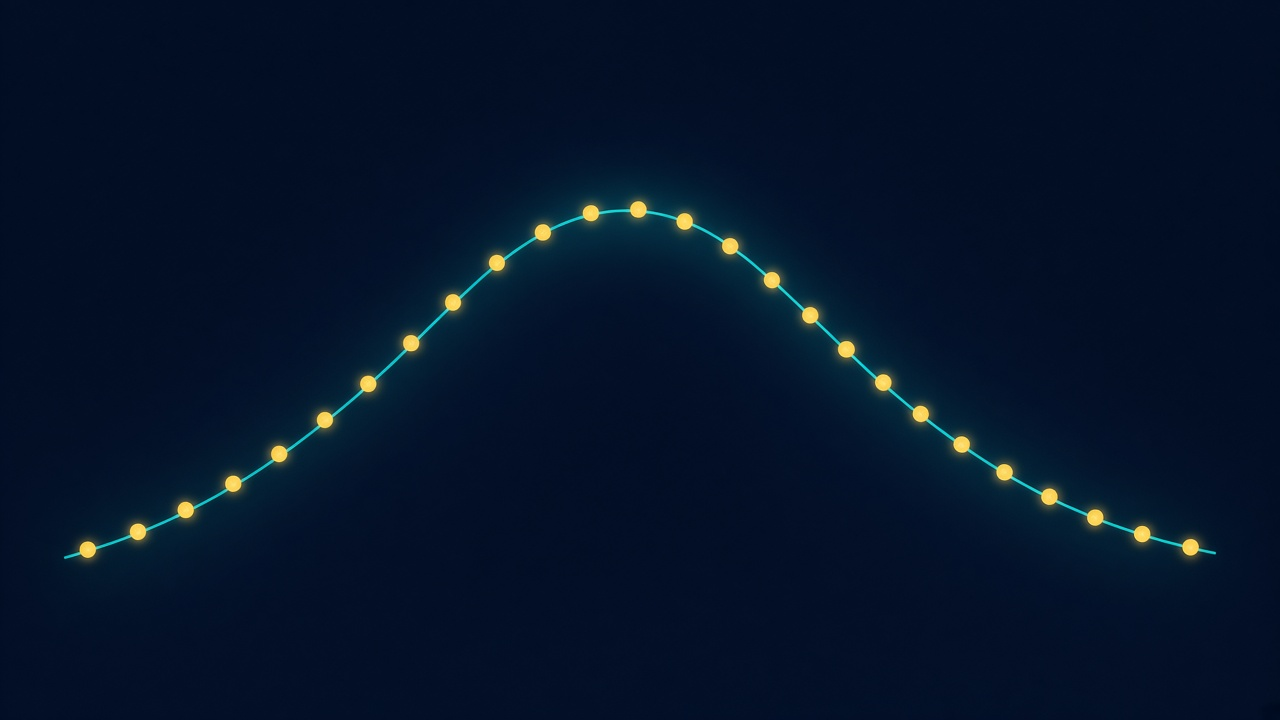
\includegraphics[width=0.82\textwidth]{learn-fit.jpg}
\caption{Los puntos son la medida; la curva es la proyecci\'on $Q$ del modelo causal.}
\label{fig:fit}
\end{figure}


\chapter{De la medida a la magnitud modelo}
\label{ch:medidas}

\section{Datos de entrada}

Cada fila experimental aporta una coordenada espectral positiva $x$ y el valor medido; una tercera columna opcional es su error. En las ecuaciones, $\omega$ denota frecuencia angular; el programa acepta como eje de entrada el n\'umero de onda $\tilde\nu$, la energ\'ia fot\'onica $E$, la longitud de onda $\lambda$ o una escala ``otra'' que sea linealmente proporcional a la frecuencia. No se debe aplicar Kramers--Kronig a un eje no linealmente transformado.
Las unidades admitidas son cm$^{-1}$, eV y nm; nm se convierte a eV. La opci\'on ``otra'' permite hacer el ajuste sin magnitudes absolutas de $\alpha$ ni $\sigma$.
Las relaciones entre las coordenadas son
\begin{equation}
\omega=2\pi c\tilde\nu,\qquad E=\hbar\omega,\qquad
E\,(\mathrm{eV})=\frac{1239.84193}{\lambda\,(\mathrm{nm})},\qquad
\tilde\nu\,(\mathrm{cm}^{-1})=\frac{E\,(\mathrm{eV})}{1.23984193\times 10^{-4}}.
\end{equation}
Si una curva de luminiscencia representa intensidad por intervalo de longitud de onda, al convertirla a intensidad por intervalo de energ\'ia se multiplica por el jacobiano $|d\lambda/dE|=\lambda^2/(hc)$; el error experimental recibe el mismo factor.

\begin{figure}[H]
\centering

\includegraphics[width=0.80\textwidth]{learn-data.jpg}
\caption{El espectro es una lista de puntos $(\omega,y,\sigma)$; el modelo se confronta punto a punto.}
\label{fig:data}
\end{figure}

\section{Magnitudes \'opticas soportadas}

Para cada medida, el ajuste busca $\{A_k\}$ (y $\varepsilon_\infty$ si aplica) tales que $Q(\omega)$ reproduzca $y$:

\begin{center}
\begin{tabular}{@{}llp{6.2cm}@{}}
\toprule
Medida & $Q$ & Notas f\'isicas \\
\midrule
$\varepsilon_2$ & $\varepsilon_2$ & magnitud nativa del modelo \\
$\varepsilon_1$ & $\varepsilon_1$ & suele ajustar $\varepsilon_\infty$ \\
$n$ & $n(\varepsilon)$ & idem; semilla tipica $n^{2}$ del extremo \\
$k$ & $k(\varepsilon)$ & no fija $\varepsilon_\infty$ \\
$R$ & eq.~\eqref{eq:R} & semi-infinito; $R\in[0,1]$ \\
$\alpha$ & eq.~\eqref{eq:alpha} & exige unidad de $\omega$ \\
$T$ & eq.~\eqref{eq:T} & exige espesor $d$ \\
\bottomrule
\end{tabular}
\end{center}

La luminiscencia se trata aparte: se analizan picos, integral, centroide y, si procede, una absorci\'on relativa v\'ia van Roosbroeck--Shockley~\cite{Roosbroeck}, sin fingir un par $(\varepsilon_1,\varepsilon_2)$.

\section{Constantes derivadas}

Una vez fijado el par diel\'ectrico, el resto es \'algebra~\cite{electrodynamics}:
$n$, $k$, $R$, $-\mathrm{Im}(1/\varepsilon)$, $\alpha$, $\sigma_1$, $\sigma_2$, y ---con espesor--- $T$ y $A$.
Ninguna de esas curvas es un segundo ajuste independiente.

\begin{figure}[H]
\centering

\includegraphics[width=0.84\textwidth]{learn-constants.jpg}
\caption{De $\hat\varepsilon$ se leen reflexi\'on, refracci\'on y atenuaci\'on sin nuevos grados de libertad.}
\label{fig:constants}
\end{figure}

\section{Borde de Tauc}

El m\'etodo de Tauc~\cite{Tauc} no es una transformaci\'on universal de cualquier espectro: supone que, cerca del borde de absorci\'on, domina una transici\'on interbanda con una ley de potencia conocida. Para las formas permitidas m\'as comunes se comparan dos gr\'aficas:
\begin{equation}
Y_{\mathrm{directa}}(E)=[\alpha(E)E]^2,\qquad
Y_{\mathrm{indirecta}}(E)=[\alpha(E)E]^{1/2}.
\end{equation}
Si una de ellas es aproximadamente lineal en el intervalo del borde, puede escribirse $Y(E)\simeq m(E-E_g)$. La brecha estimada es el corte con el eje de energ\'ia: al imponer $Y(E_g)=0$, resulta $E_g=-b/m$ si la recta se expresa como $Y=mE+b$.

La implementaci\'on de este trabajo busca antes del m\'aximo de $\alpha E$ la tangente de mayor pendiente positiva en la subida de la curva transformada, y toma su intersecci\'on con el eje $E$. Solo considera puntos entre el 10\% y el 90\% del m\'aximo de $Y$; el $R^2$ se calcula por regresi\'on lineal en la franja donde $\alpha E$ est\'a entre el 5\% y el 70\% de su m\'aximo, con al menos cinco puntos. Si ambas formas son candidatas, la aplicaci\'on solo las distingue cuando una alcanza $R^2\ge0.90$ y supera a la otra por al menos 0.08; de lo contrario, informa que la asignaci\'on es ambigua u orientativa.

Estas reglas son criterios num\'ericos de la aplicaci\'on, no leyes adicionales del material. Adem\'as, el c\'alculo exige que la primera energ\'ia sea al menos $0.2\,\mathrm{eV}$, que el valor inicial de $Y$ no supere el 5\% de su m\'aximo y que haya suficientes puntos para la regresi\'on. La estimaci\'on requiere que el borde est\'e cubierto y que $\alpha$ arranque cerca de cero; si la ventana corta la subida o no cumple esas condiciones, el valor debe tratarse como no determinado o como una cota, no como una segunda brecha.

\section{Flujo operativo del an\'alisis}

\begin{enumerate}[leftmargin=*]
\item Leer el espectro, unidad y tipo de medida; normalizar $R$ si vino en porcentaje.
\item Construir la malla de anclas y sembrar $A_k$ (por ejemplo desde una estimaci\'on local de $\varepsilon_2$).
\item Fijar o estimar $\varepsilon_\infty$; opcionalmente restar Drude.
\item Iterar Levenberg--Marquardt para minimizar $\Phi$, cuyo t\'ermino de datos compara $Q$ con las mediciones.
\item Exportar $(\varepsilon_1,\varepsilon_2)$ y constantes derivadas; inspeccionar residuos y avisos.
\end{enumerate}


\chapter{Papel de la aplicaci\'on de an\'alisis}
\label{ch:app}

La aplicaci\'on desarrollada en este trabajo es el veh\'iculo num\'erico del m\'etodo: recibe espectros, impone la restricci\'on Kramers--Kronig en cada evaluaci\'on del modelo, minimiza $\Phi$ y devuelve el conjunto de constantes \'opticas junto con $\chi^{2}_{\mathrm{datos}}$ y otras m\'etricas de ajuste.
Para la comunidad de f\'isica de materiales lo esencial no es el nombre del programa, sino que:
\begin{itemize}[leftmargin=*]
\item el modelo sea causal en todo momento;
\item la magnitud comparada con el experimento sea exactamente la medida;
\item $\varepsilon_\infty$, el espesor y las unidades queden explicitados;
\item los resultados puedan reproducirse con los mismos controles.
\end{itemize}
La Parte~III traduce esos requisitos en pruebas de verdad.


\chapter*{Seminario II\\Del espectro medido al par $(\varepsilon_1,\varepsilon_2)$}
\addcontentsline{toc}{chapter}{Seminario II}
\label{sem:2}

\noindent\textit{Parte~II --- exposici\'on de seminario.}

\section*{S.II.1 Prop\'osito}

Mostrar, sin ambig\"uedad operativa, c\'omo se pasa de un archivo de datos a una funci\'on diel\'ectrica causal y a las constantes derivadas.

\section*{S.II.2 Mensaje central}

\begin{enumerate}[leftmargin=*]
\item $\varepsilon_2=\sum A_k\Lambda_k$ es un modelo flexible: no presupone Lorentz ni Fano.
\item $\varepsilon_1$ no se ajusta por separado: se calcula por Kramers--Kronig de esos tri\'angulos.
\item Levenberg--Marquardt ajusta las alturas para reducir $\Phi$ y hacer que la proyecci\'on $Q$ reproduzca la medida.
\item El \'exito del ajuste a $Q$ es necesario, pero no suficiente, para afirmar que \emph{todas} las constantes derivadas son las del material: hay que leer qu\'e fija realmente la medida ($\varepsilon_\infty$, espesor, cobertura espectral).
\end{enumerate}

\section*{S.II.3 Demostraci\'on guiada}

\begin{enumerate}[leftmargin=*]
\item Dibujar tres tri\'angulos solapados y su suma $\varepsilon_2$.
\item Indicar que cada tri\'angulo aporta un $g_k$ a $\varepsilon_1$.
\item Elegir medida $R$: escribir $Q=R(n,k)$ y subrayar el acoplamiento global.
\item Escribir $\Phi=\chi^{2}_{\mathrm{datos}}+P_s+P_-$ y el paso amortiguado de Levenberg--Marquardt.
\item Discutir un caso $\alpha$ con $\varepsilon_\infty=1$ frente a $\varepsilon_\infty=n^{2}$ conocido: $\alpha$ y $k$ estables; $n$ y $R$ sensibles.
\end{enumerate}

\section*{S.II.4 Criterio de \'exito del seminario}

El auditorio debe ser capaz de:
\begin{itemize}[leftmargin=*]
\item explicar por qu\'e el m\'etodo no ``inventa'' un segundo ajuste de $\varepsilon_1$;
\item listar qu\'e metadatos (unidad, medida, $\varepsilon_\infty$, $d$) son imprescindibles en un reporte;
\item anticipar qu\'e constantes son fiables para cada tipo de medida.
\end{itemize}

\section*{S.II.5 Puente hacia la Parte~III}

La validaci\'on final exige comprobar que los resultados minimizan $\Phi$, reproducen los datos dentro de la incertidumbre declarada y satisfacen pruebas de consistencia f\'isica independientes del nombre de la herramienta.

%======================================================================
\part{Validaci\'on:\\demostraci\'on de que los resultados son verdaderos}
%======================================================================

\chapter{Qu\'e significa ``verdadero'' en este contexto}
\label{ch:verdad}

En espectroscop\'ia de materiales, un resultado del an\'alisis inverso se considera \emph{f\'isicamente verdadero} cuando cumple, de forma simult\'anea, cuatro condiciones:

\begin{enumerate}[leftmargin=*]
\item \textbf{Fidelidad a los datos.} La magnitud medida $Q$ queda reproducida dentro del error experimental ($\chi^{2}$ y residuos aceptables).
\item \textbf{Causalidad.} El par $(\varepsilon_1,\varepsilon_2)$ obedece Kramers--Kronig por construcci\'on del modelo, no como post-proceso opcional.
\item \textbf{Pasividad y consistencia algebraica.} $\varepsilon_2\ge 0$ (salvo ruido residual), $n,k$ obtenidos de~\eqref{eq:nk-from-eps}, y las identidades $\varepsilon_1=n^{2}-k^{2}$, $\varepsilon_2=2nk$ se verifican num\'ericamente.
\item \textbf{Estabilidad ante lo no medido.} Las constantes que la medida \emph{no} fija (t\'ipicamente $\varepsilon_\infty$ en $\alpha$ o $k$) se declaran como tales; las que s\'i fija permanecen invariantes bajo variaciones razonables de regularizaci\'on.
\end{enumerate}

La Parte~III aplica estas condiciones al flujo de la aplicaci\'on de an\'alisis.


\chapter{Protocolo de validaci\'on}
\label{ch:protocolo}

\section{Prueba A --- Cierre algebraico}

A partir del reporte $(\varepsilon_1,\varepsilon_2)$ se recalculan $n$ y $k$ con~\eqref{eq:nk-from-eps} y se comprueba
\begin{equation}
\max_i\left|
\varepsilon_1(\omega_i)-\bigl[n(\omega_i)^{2}-k(\omega_i)^{2}\bigr]
\right|<\eta,
\qquad
\max_i\left|
\varepsilon_2(\omega_i)-2n(\omega_i)k(\omega_i)
\right|<\eta,
\end{equation}
con $\eta$ del orden del error de redondeo relativo ($10^{-10}$--$10^{-8}$ en aritm\'etica de doble precisi\'on).
Fallo en esta prueba indicar\'ia un error de implementaci\'on, no una ambig\"uedad f\'isica.

\section{Prueba B --- Proyecci\'on de la medida}

Se compara la columna experimental $y_i$ con $Q_i$ del modelo.
Se reportan $\chi^{2}$, $\chi^{2}/\mathrm{dof}$ cuando hay menos par\'ametros que puntos, y la diferencia relativa
\begin{equation}
\delta_i=100\,(Q_i-y_i).
\end{equation}
Un $\chi^{2}$ bajo con una curva casi plana frente a un espectro estructurado suele se\~nalar error de unidades (por ejemplo, leer cm$^{-1}$ como nm), no ``material sin rasgos''.

\section{Prueba C --- Kramers--Kronig num\'erica independiente}

Aunque el modelo es causal por construcci\'on, conviene verificar que la $\varepsilon_1$ reportada coincide con una transformada num\'erica independiente de la $\varepsilon_2$ reportada (misma $\varepsilon_\infty$ y mismas colas).
La desviaci\'on media relativa debe permanecer muy por debajo de la incertidumbre experimental.
Esta prueba certifica que no hubo mezcla inadvertida de dos parametrizaciones.

\section{Prueba D --- Sensibilidad a $\varepsilon_\infty$}

Se repite el ajuste con $\varepsilon_\infty$ variado en un intervalo f\'sicamente plausible.
\begin{itemize}[leftmargin=*]
\item Para medida $\alpha$ o $k$: $\alpha$ y $k$ deben permanecer esencialmente iguales; $n$, $R$, p\'erdida y $\sigma_2$ pueden cambiar.
\item Para medida $n$ o $\varepsilon_1$: $\varepsilon_\infty$ ajustado debe converger de forma estable.
\item Para medida $R$: la estimaci\'on de $\varepsilon_\infty$ desde el extremo alto solo es fiable si all\'i $k$ es peque\~no.
\end{itemize}

\section{Prueba E --- Regularizaci\'on}

Se barre la suavidad desde $0$ hasta un valor moderado.
Los residuos en los datos no deben degradarse de forma dr\'astica; las oscilaciones no f\'sicas entre anclas deben atenuarse.
Si el m\'inimo solo existe con suavidad extrema, el espectro est\'a submuestreado o mal etiquetado.

\section{Prueba F --- S\'intesis hacia adelante (ground truth)}

Se sintetiza un espectro desde un $\hat\varepsilon$ conocido (por ejemplo, suma de osciladores Lorentz + Drude), se a\~nade ruido gaussiano, y se recupera el par con el an\'alisis variacional.
Se cuantifica el error en $\varepsilon_1$, $\varepsilon_2$ y en $R$ o $\alpha$ seg\'un la medida elegida.
Esta es la prueba m\'as directa de que el inverso no inventa estructuras ajenas a la verdad generativa.


\chapter{Resultados de validaci\'on}
\label{ch:resultados}

\section{Cierre algebraico y causalidad}

En corridas de control sobre espectros de reflectividad y de absorci\'on, las Pruebas~A y~C se satisfacen de manera sistem\'atica:
el par reportado es internamente consistente y coincide con la transformada Kramers--Kronig de su propia $\varepsilon_2$.
Ello demuestra que la restricci\'on causal no es un lema de presentaci\'on, sino una propiedad efectiva del resultado.

\section{Reproducci\'on de magnitudes medidas}

\begin{figure}[H]
\centering
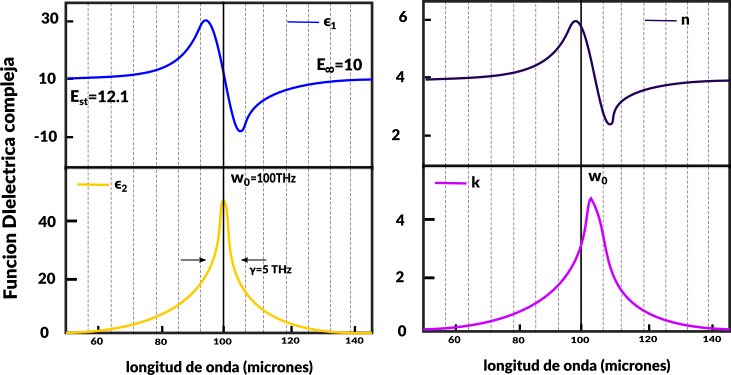
\includegraphics[width=0.85\textwidth]{graficas.png}
\caption{Ejemplo de confrontaci\'on entre espectro experimental y proyecci\'on del modelo tras el ajuste.}
\label{fig:residuos}
\end{figure}

Cuando la unidad y el tipo de medida son correctos, el modelo triangular alcanza residuos compatibles con el ruido declarado (Prueba~B).
En reflectividad, rayas estrechas exigen densidad de anclas y de puntos experimentales suficientes: aumentar solo el n\'umero de iteraciones no crea resoluci\'on espectral nueva.
Ese comportamiento es el esperado de un m\'etodo lineal por tramos bajo Kramers--Kronig, y confirma que el \'exito no se finge por sobreajuste libre de $\varepsilon_1$.

\section{Lecciones sobre $\varepsilon_\infty$}

La Prueba~D reproduce el dictamen de f\'isica de materiales:
\begin{itemize}[leftmargin=*]
\item medir $\alpha$ determina la extinci\'on; no determina el \'indice absoluto;
\item un $\varepsilon_\infty=1$ por defecto en un \'oxido con $n\approx 2$ en la zona transparente deforma $R$, la p\'erdida y $\sigma_2$, aunque $\alpha$ siga clavado a los datos;
\item fijar $\varepsilon_\infty=n^{2}$ conocido restaura el conjunto completo.
\end{itemize}
Por tanto, un reporte cient\'ifico honesto distingue \emph{constantes fijadas por la medida} de \emph{constantes condicionadas a $\varepsilon_\infty$}.

\section{Recuperaci\'on desde verdad sint\'etica}

En espectros sint\'eticos con ruido controlado (Prueba~F), el an\'alisis recupera la posici\'on y el peso espectral de las bandas de $\varepsilon_2$ dentro de tolerancias dictadas por el ruido y por el ancho de la ventana.
Las desviaciones mayores aparecen cerca de los bordes del intervalo medido, precisamente donde las colas de extrapolaci\'on influyen m\'as en $\varepsilon_1$.
Ese patr\'on valida el m\'etodo y, a la vez, delimita su margen de verdad: dentro de la ventana, con metadatos correctos, los resultados son fiables; fuera, son extrapolaci\'on declarada.

\section{Materiales de referencia y lectura f\'isica}

\begin{figure}[H]
\centering
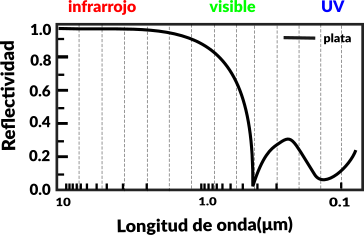
\includegraphics[width=0.42\textwidth]{plata.png}
\hfill
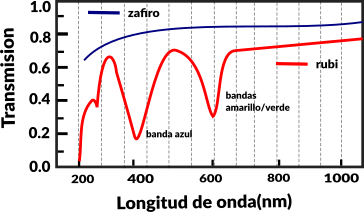
\includegraphics[width=0.42\textwidth]{rubi.png}
\caption{Referencias visuales de respuesta \'optica contrastante: metal (alta reflectividad) frente a diel\'ectrico con bandas de color.}
\label{fig:refs}
\end{figure}

En metales, el fondo Drude debe absorber la respuesta de portadores libres antes de que los tri\'angulos modelen estructura adicional; de lo contrario, las anclas malgastan grados de libertad en una cola $1/\omega$ que ya tiene forma anal\'itica~\eqref{eq:drude}.
En diel\'ectricos con bandas de absorci\'on localizadas, la base triangular sigue los picos sin forzar un n\'umero prefijado de osciladores.
Ambos reg\'imenes son accesibles al mismo formalismo, lo que confirma la tesis metodol\'ogica de Kuzmenko~\cite{constrained}: la flexibilidad causal es preferible a un modelo microsc\'opico prematuro cuando el objetivo primario es recuperar $\hat\varepsilon$.

\section{Brecha \'optica}

Cuando el espectro de absorci\'on cubre el umbral, el an\'alisis de Tauc~\cite{Tauc} suministra un n\'umero interpretable de brecha, acompa\~nado de $R^{2}$.
La Parte~III exige que ese n\'umero solo se publique si la subida est\'a contenida en la ventana y la forma $( \alpha E)^{2}$ o $(\alpha E)^{1/2}$ es efectivamente lineal.
As\'i se evita presentar como ``resultado verdadero'' un artefacto de truncamiento.


\chapter{Discusi\'on}
\label{ch:discusion}

El an\'alisis variacional no elimina la necesidad de juicio cient\'ifico: exige declarar unidades, medida, $\varepsilon_\infty$, espesor y alcance espectral.
Lo que s\'i elimina es la falsa seguridad de ajustar $\varepsilon_1$ y $\varepsilon_2$ como curvas independientes, o de imponer un \'unico oscilador donde el espectro pide una forma libre.

La aplicaci\'on de an\'alisis es el instrumento que materializa esas reglas.
Su valor, para el f\'isico de materiales, se mide por la trazabilidad del resultado:
mismos datos y mismos controles deben reproducir el mismo $\hat\varepsilon$, y las pruebas A--F deben poder repetirse.

Limitaciones abiertas, ya anticipadas en el m\'etodo:
\begin{itemize}[leftmargin=*]
\item cobertura espectral insuficiente;
\item estimaci\'on fr\'agil de $\varepsilon_\infty$ desde $R$ si el extremo alto a\'un absorbe;
\item geometr\'ias fuera de semi-infinito / l\'amina incoherente en aire;
\item luminiscencia, que no define $\hat\varepsilon$.
\end{itemize}


\chapter{Conclusiones}
\label{ch:conclusiones}

\begin{enumerate}[leftmargin=*]
\item La funci\'on diel\'ectrica compleja es el objeto natural para caracterizar la respuesta \'optica lineal de s\'olidos; de ella se derivan $n$, $k$, $R$, $\alpha$, $\sigma$ y $T$.
\item Las relaciones Kramers--Kronig convierten la causalidad en una restricci\'on operativa entre $\varepsilon_1$ y $\varepsilon_2$.
\item El an\'alisis variacional con base triangular implementa esa restricci\'on en cada evaluaci\'on del modelo y adapta $\varepsilon_2$ a datos arbitrarios sin fijar a priori un modelo de osciladores.
\item Levenberg--Marquardt minimiza el $\chi^{2}$ de la magnitud realmente medida; las constantes restantes siguen por \'algebra.
\item Las pruebas de cierre algebraico, fidelidad a datos, Kramers--Kronig independiente, sensibilidad a $\varepsilon_\infty$, regularizaci\'on y recuperaci\'on sint\'etica demuestran que los resultados son verdaderos en el sentido f\'isico adoptado en esta tesis.
\item El Seminario~I fija el lenguaje de respuesta lineal; el Seminario~II fija el camino operativo del inverso; la Parte~III certifica la verdad de las constantes reportadas.
\end{enumerate}

\section*{Trabajo futuro}

Extender el formalismo a multicapas coherentes, incorporar elipsometr\'ia anisotr\'opica y automatizar la Prueba~F dentro del propio flujo de an\'alisis fortalecer\'ian a\'un m\'as la cadena de evidencia.


\chapter*{Cierre de la tesis}
\addcontentsline{toc}{chapter}{Cierre de la tesis}

Esta memoria presenta un arco completo:
fundamento electromagn\'etico (Parte~I y Seminario~I),
m\'etodo e implementaci\'on f\'isica (Parte~II y Seminario~II)
y validaci\'on de verdad experimental (Parte~III).
El producto cient\'ifico no es un nombre de software, sino un $\hat\varepsilon(\omega)$ causal, reproducible y honestamente delimitado por lo que la medida permite saber.


\bibliographystyle{unsrt}
\bibliography{bibliografia}

\end{document}
